% Created 2015-01-28 Mit 18:22
\documentclass[11pt, a4paper,titlepage]{article}
\usepackage[utf8]{inputenc}
\usepackage[T1]{fontenc}
\usepackage{fixltx2e}
\usepackage{graphicx}
\usepackage{longtable}
\usepackage{float}
\usepackage{wrapfig}
\usepackage{soul}
\usepackage{textcomp}
\usepackage{marvosym}
\usepackage{wasysym}
\usepackage{latexsym}
\usepackage{amssymb}
\usepackage{hyperref}
\tolerance=1000
\usepackage[left=2.35cm, right=3.35cm, top=3.35cm, bottom=3.35cm]{geometry}
\usepackage[utf8]{inputenc}
\usepackage[english]{babel}
\usepackage{graphicx}
\usepackage{titlesec}
\usepackage{chemfig}
\providecommand{\alert}[1]{\textbf{#1}}

\title{}
\author{Cedric Lood}
\date{\today}
\hypersetup{
  pdfkeywords={},
  pdfsubject={},
  pdfcreator={Emacs Org-mode version 7.9.3f}}

\begin{document}



\setlength{\parskip}{0pt}%
\setlength{\parindent}{0pt}%
\renewcommand{\thesubsubsection}{\alph{subsubsection}.)}
\begin{titlepage}
  \begin{center}
    
    
\includegraphics[scale=1.5]{Figures/kuleuven_logo.pdf}~\\[4.5cm]
    
    \textsc{\Large Basics of biological chemistry}\\[0.5cm]
    
    % Title
    \rule{\linewidth}{0.3mm}\\[0.4cm]
    {\huge \bfseries Assignment} \\[0.4cm]
    {\large January 2015 Finals} \\[0.4cm]
    \rule{\linewidth}{0.3mm}\\[1.5cm]
    
    % Author and supervisor
    \begin{minipage}{0.4\textwidth}
      \begin{flushleft} \large
        \emph{Author:}\\
        Cedric \textsc{Lood}\\
      \end{flushleft}
    \end{minipage}
    \begin{minipage}{0.4\textwidth}
      \begin{flushright} \large
        \emph{Supervisors:} \\
        Prof. J. \textsc{Vanderleyden}\\
        dr. H. \textsc{Steenackers}\\
        Prof. B. \textsc{Sels}\\
        Prof. J. \textsc{Vanderleyden}
      \end{flushright}
    \end{minipage}
    
    \vfill
    
    % Bottom of the page
    {\large \today}
    
  \end{center}
\end{titlepage}

\setcounter{tocdepth}{3}
\tableofcontents
\clearpage



\section{Prof. J. Vanderleyden – dr. H. Steenackers}
\label{sec-1}
\subsection{Chemical reaction equation}
\label{sec-1-1}


Consider the following reaction: (NH$_{4}$)$_{2}$CO$_{3}$ +  Zn(NO$_{3}$)$_{2}$ →  NH$_{4}$NO$_{3}$ + ZnCO$_{3}$
\subsubsection{Balance the equation}
\label{sec-1-1-1}

(NH$_{4}$)$_{2}$CO$_{3}$ +  Zn(NO$_{3}$)$_{2}$ →  2 NH$_{4}$NO$_{3}$ + ZnCO$_{3}$
\subsubsection{Reactants and products}
\label{sec-1-1-2}

\texttt{Q:} Name all reactants and reaction products.

\texttt{A:}
\begin{itemize}
\item (NH$_{4}$)$_{2}$CO$_{3}$ : Ammonium carbonate
\item Zn(NO$_{3}$)$_{2}$ : Zinc nitrate
\item NH$_{4}$NO$_{3}$ : Ammonium nitrate
\item ZnCO$_{3}$ : Zinc carbonate
\end{itemize}
\subsubsection{Lewis structure, VESPR}
\label{sec-1-1-3}

\texttt{Q:} Construct the Lewis structures of the polyatomic ions you recognize
and predict their molecular structure using the VSEPR theory.

\texttt{A:}
\begin{itemize}
\item Lewis Structure of the ions:
\end{itemize}
\renewcommand{\arraystretch}{1.5}
\begin{tabular}{ c | c | c | c}
Ammonium & Carbonate & Zinc & Nitrate  \\
\hline
\chemfig{N^{+}(-[:0]H)(-[:90]H)(-[:180]H)(-[:270]H)} &
\chemfig{\lewis{3:5:,O}=C(-[1]\lewis{3:1:7:,O}^{-})(-[7]\lewis{1:7:5:,O}^{-})} &
\chemfig{\lewis{4:,Zn^{2+}}} &
\chemfig{\lewis{3:5:,O}=N^{+}(-[1]\lewis{3:1:7:,O}^{-})(-[7]\lewis{1:7:5:,O}^{-})}\\
\end{tabular}

\begin{itemize}
\item Molecular structure prediction:
\end{itemize}
\renewcommand{\arraystretch}{1.5}
\begin{tabular}{ c | c | c | c}
Ammonium & Carbonate & Zinc & Nitrate  \\
\hline
\chemfig{N^{+}(-[2]H)(-[5]H)(<[6]H)(<:[7]H)} &
\chemfig{O=C(-[1]O^{-})(-[7]O^{-})} &
\chemfig{Zn^{2+}} &
\chemfig{O=N^{+}(-[1]O^{-})(-[7]O^{-})}\\
\end{tabular}
\subsubsection{Oxidation states}
\label{sec-1-1-4}

\texttt{Q:} Determine the oxidation state of all the atoms in all the
compounds. Is this an oxidation-reduction reaction?

\texttt{A:} Ammonium Carbonate and Zinc Nitrate (the reactants) are very soluble
in water and will thus move freely. The Zinc and Carbonate ions will
then precipitate.

\begin{itemize}
\item Zn has an oxidation state of 2:  Zn →  Zn$^{\mathrm{2+}}$ + 2 e$^{-}$
\item (CO$_{3}$) has an oxidation state of 4: (CO$_{3}$)$^{\mathrm{2-}}$ + 2 e$^{-}$ → CO$_{3}$
\end{itemize}
\subsubsection{Mass}
\label{sec-1-1-5}

\texttt{Q:} How many grams of ZnCO3 can be prepared from 400g Zn(NO3)2 by
using sufficient(NH4)2CO3?

\texttt{A:} Let's start by computing the molecular weight of the 2 reactants:

\begin{description}
\item[Molecular weigth of Zn(NO$_{3}$)$_{2}$] 189.36 g/mol
\item[Molecular weigth of (NH$_{4}$)$_{2}$CO$_{3}$] 96.09 g/mol
\end{description}

Given that there are 400g of Zn(NO$_{3}$)$_{2}$, we can calculate the
number of moles of reactant (and ignore that of (NH$_{4}$)$_{2}$CO$_{3}$
since it is in excess):

\begin{description}
\item[Moles of Zn(NO$_{3}$)$_{2}$] 400 g / 189.36 g/mol = 2.11237 moles
\end{description}

From this last figure, we can infer that the number of moles of
ZnCO$_{3}$ will be 2.11237. Given the molecular mass of ZnCO$_{3}$, we can
compute the amount of ZnCO$_{3}$ produced to be: 2.11237 mol * 125.3889
g/mol = 264.8678 g.
\subsection{DNA sequence analysis}
\label{sec-1-2}


The following diagram shows part of a template DNA strand, with
sections X,Y and Z being the exons of a gene:


\begin{verbatim}
5'                        3'
GTA GGT TGT ATC GAT GGT CAT
---     -------         ---
 X         Y             Z
\end{verbatim}
\subsubsection{DNA Replication}
\label{sec-1-2-1}

\texttt{Q:} What is the corresponding sequence on the new daughter strand
made from the given parent strand during replication?

\texttt{A:} Given the principle of base pairing, we can determine the daughter
sequence to be (here in the 3' to 5' direction):


\begin{verbatim}
5'                        3'
GTA GGT TGT ATC GAT GGT CAT
CAT CCA ACA TAG CTA CCA GTA
3'                        5'
\end{verbatim}
\subsubsection{Translated Protein}
\label{sec-1-2-2}

\texttt{Q:} What polypeptide sequence will be synthesized from the given template
DNA? Give a short overview of the different processes (and enzymes)
involved in the synthesis of polypeptides from template DNA. Where in
the cell do these processes take place?

\texttt{A:} The synthesized polypeptide will consist of the amino acids \texttt{VCIH}. 
\subsubsection{Mutated exon}
\label{sec-1-2-3}

\texttt{Q:} What polypeptide sequence will be synthesized if the ATC in exon
Y is mutated to TTC? What polypeptide sequence will be synthesized if
the ATC in exon Y is mutated to ATG? Which of those substitution
mutations is likely to be more harmful? Why?

\texttt{A:}
\subsubsection{Interactions with antibiotics}
\label{sec-1-2-4}

\texttt{Q:} Which steps in polypeptide synthesis are affected by resp. the
macrolide antibiotics and the tetracycline antibiotics?

\texttt{A:}
\subsubsection{Comparison of error rates}
\label{sec-1-2-5}

\texttt{Q:} The error rate in RNA synthesis is much higher than the error rate
of DNA replication. What is the origin of this difference? Motivate
why this is not a serious problem.

\texttt{A:}
\subsection{tRNA 3D-Structure}
\label{sec-1-3}

\texttt{Q:} All tRNA molecules have a particular 3D-structure. Which
functional groups and which chemical bonds/interactions contribute to
this particular structure? Why is this particular structure of
importance for the biological function?

\texttt{A:}
\section{Prof. B. Sels}
\label{sec-2}
\subsection{Biopolymer organisation}
\label{sec-2-1}

\texttt{Q:} The course and the textbook systematically organize four important
biopolymers mainly according to their chemical structure. Attempt a
complete reorganization of the various biopolymer structures (and
subfamilies!) according to the following three physiological
functions: energy, structure, and communication. Explain the
physiological function of each biopolymer type with regard to its
chemical structure and/or physical properties.

\texttt{A:}
\subsection{Chemical structure of proteins and proteins separation}
\label{sec-2-2}

\texttt{Q:} Draw the chemical structure of the following two oligopeptide
structures, a) Gln-Ser-Lys-Lys-Ser and b) Cys-Asp-Asp-Glu-Lys,
determine its net charge in physiological conditions. How would you
separate the two peptides ?  

\texttt{A:}
\subsection{Chemical structure of disaccharides}
\label{sec-2-3}

\texttt{Q:} Draw the chemical structure of the following disaccharides: a)
the $\beta$-anomer of $\alpha$(1→6)galactoglucose and b)
$\beta$,$\alpha$(1→2)glucofructose.

\texttt{A:}
\section{Prof. D. De Vos}
\label{sec-3}

Considering the following molecule:

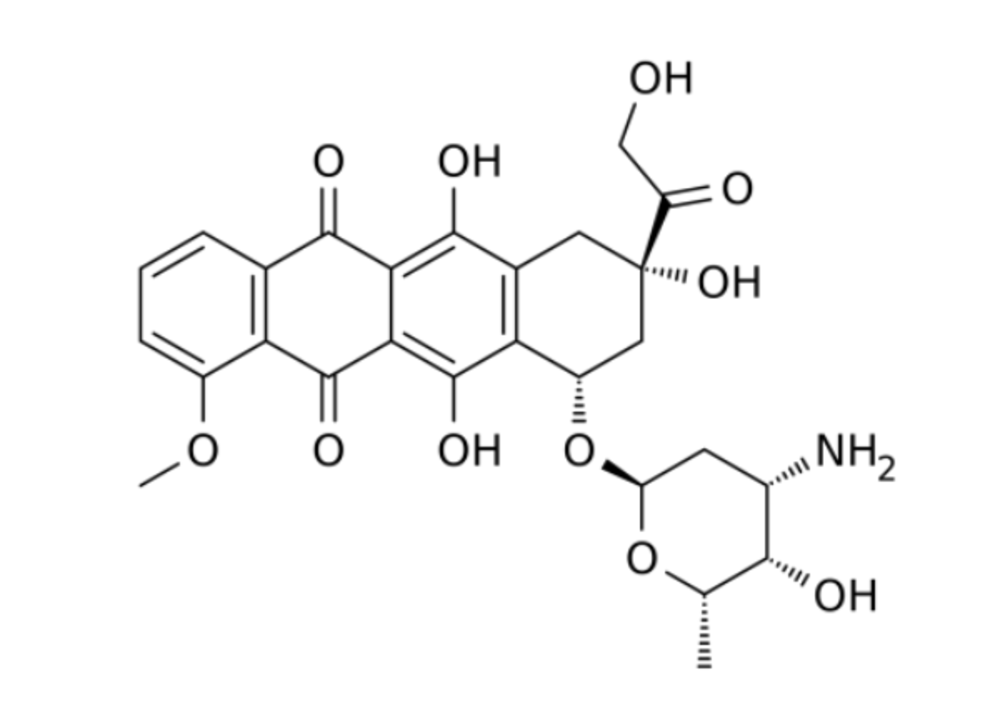
\includegraphics[width=10cm]{./Figures/Part3MoleculeRaw.pdf}
\subsection{Functional groups}
\label{sec-3-1}

\texttt{Q:} Name all functional groups

\texttt{A:} See annoted figure below

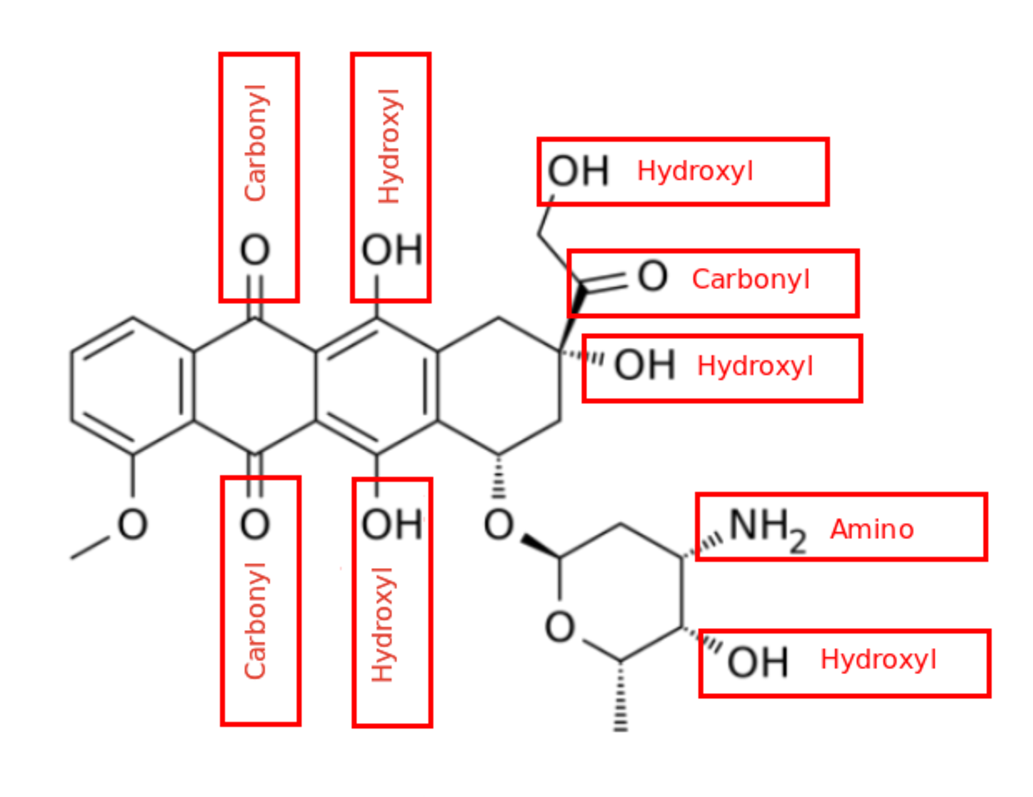
\includegraphics[width=10cm]{./Figures/Part3MoleculeFunctionalGroups.pdf}
\subsection{Water and oil solubility factors}
\label{sec-3-2}

\texttt{Q:} Indicate which groups make the molecule rather water-soluble
than oil-soluble

\texttt{A:} The following groups can partake in hydrogen bonds with water
molecules and increase the solubility of the molecule in water :

\begin{itemize}
\item Hydroxyl groups (5 of them)
\item Carbonyl groups (3 of them)
\item Amino group (1 present)
\end{itemize}

\end{document}
